\documentclass[paper=a4, fontsize=11pt]{article}

\usepackage[T1]{fontenc}
\usepackage[english]{babel}
\usepackage{amsmath,amsfonts,amsthm}

\usepackage[margin=0.5in, top=0.2in]{geometry}

\usepackage{subfig}
\usepackage{epsfig}
\usepackage{graphicx}
\usepackage{color}
\usepackage{epstopdf}
\usepackage{cancel}
\usepackage{hyperref}
%\setkomafont{caption}{\footnotesize\sf}
%\setkomafont{captionlabel}{\usekomafont{caption}}
\usepackage{caption}
%\usepackage{subcaption}

\usepackage[backend=bibtex]{biblatex}

\graphicspath{{./fig/}}

\addbibresource{tagirov.bib}

\numberwithin{equation}{section} 
\numberwithin{figure}{section} 
\numberwithin{table}{section} 

\setlength\parindent{20pt}

\newcommand{\mr}[1]{\mathrm{#1}}
\newcommand{\mb}[1]{\mathbf{#1}}
\newcommand{\p}{\partial}

\def\araa{Annual Review of Astronomy and Astrophysics}
\def\nat{Nature}

%----------------------------------------------------------------------------------------
%	TITLE
%----------------------------------------------------------------------------------------

\newcommand{\horrule}[1]{\rule{\linewidth}{#1}}
\newcommand{\rom}[1]{\uppercase\expandafter{\romannumeral #1\relax}}

\begin{document}

%\setcounter{page}{1}
\setcounter{section}{0}
\section{Introduction}
This project is concerned with the identification and studying of the solar active regions,
which are concentrations of relatively high magnetic field on the solar surface.
One of the types of active regions is a sun-spot.
Sun-spots (when they are present) are seen as the isolated dark areas on the solar disk when the latter
is observed in the visible or IR wavelengths.
The other type is faculae which are seen in the magnetic field images of the Sun.
In actuality, there are more types of active regions, but for the purposes of the project this basic
division into spots and faculae will suffice.

In this project we will work with the high-resolution (4096 $\times$ 4096 pixels) intensity images and magnetograms 
of the solar disk obtained with the Helioseismic and Magnetic Imager (HMI) onboard Solar Dynamics Observatory (SDO).
An example of these data is shown in Fig.~\ref{fig:sdo_img}.
\begin{figure*}[h!]
\centering
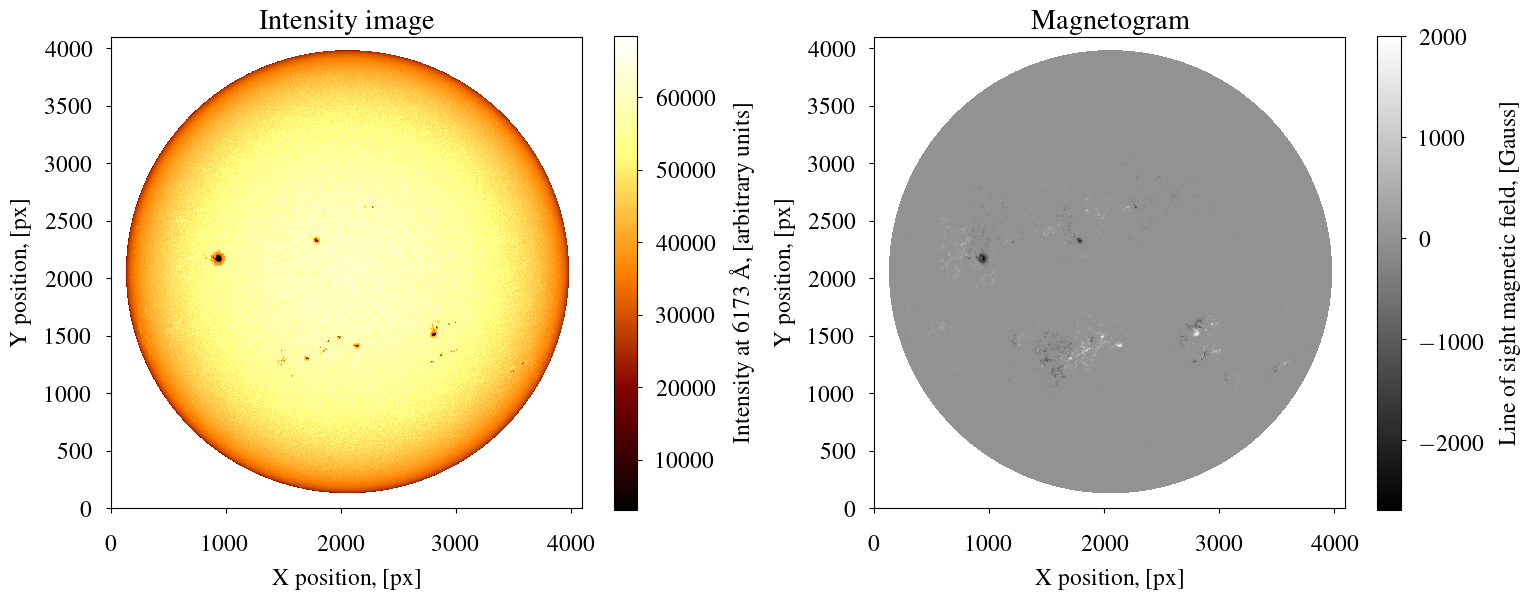
\includegraphics[scale=0.495]{sdo_img}
\caption[]{The HMI/SDO intensity image (left panel) and magnetogram (right panel) for 16.11.2013.}
\label{fig:sdo_img}
\end{figure*}
Each pixel of the intensity image contains the intensity (in arbitrary units) at 6173 \AA\ wavelength and
each pixel of the magnetogram contains the line-of-sight component of magnetic field in Gauss.
Since both spots and faculae manifest themselves in magnetograms, but only spots show the darkening in the intensity
images, analyzing these two types of data allows to identify spots and faculae on the solar disk.

The core of this project can be boiled down to the following goals:
\begin{itemize}
\item see how sun-spots are different from facular structures in terms of their morphology;
\item find out what the strengths of typical magnetic fields in faculae and the inner parts of sun-spots are;
\item find out what the typical sizes of sun-spots are;
\end{itemize}
In what follows, the main aspects of the analysis will be demonstrated using the images shown in Fig.~\ref{fig:sdo_img}.
Where needed the references to \texttt{python 3.6.0} functions will be made.
It should be mentioned at the outset that we will restrict ourselves by not considering the
outer parts of the solar disk ($r / R_\odot < 0.953$), the so-called limb, because the analysis is greatly hindered there
by the projection effect.
The identification of active regions in the images starts with finding the image pixels in which we reliably measure the signal.

\section{Intensity images}
\subsection{Center-to-Limb Variation}
Fig.~\ref{fig:int_scan} shows the scan of the intensity image through the biggest sun-spot within $r = 0.953R\odot$ circumference.
The intensity values are stored in a \texttt{fits} format file.
The access to them as well as to the coordinates of the solar disk center $(x_0, y_0)$ 
and solar radius $R_\odot$, which we will need in the analysis,
can be carried out in the following way:
\begin{verbatim}
    >>> from astropy.io import fits

    >>> hdulist_int = fits.open('/path/to/intensity/fits/file')

    >>> hdu_int = hdulist_int[0]

    >>> I = hdu_int.data # hdu_int.data is a 2D-array

    >>> x0 = hdu_int.header['X0']; y0 = hdu_int.header['Y0']

    >>> rsun = hdu_int.header['R_SUN']
\end{verbatim}
\begin{figure*}[h!]
\centering
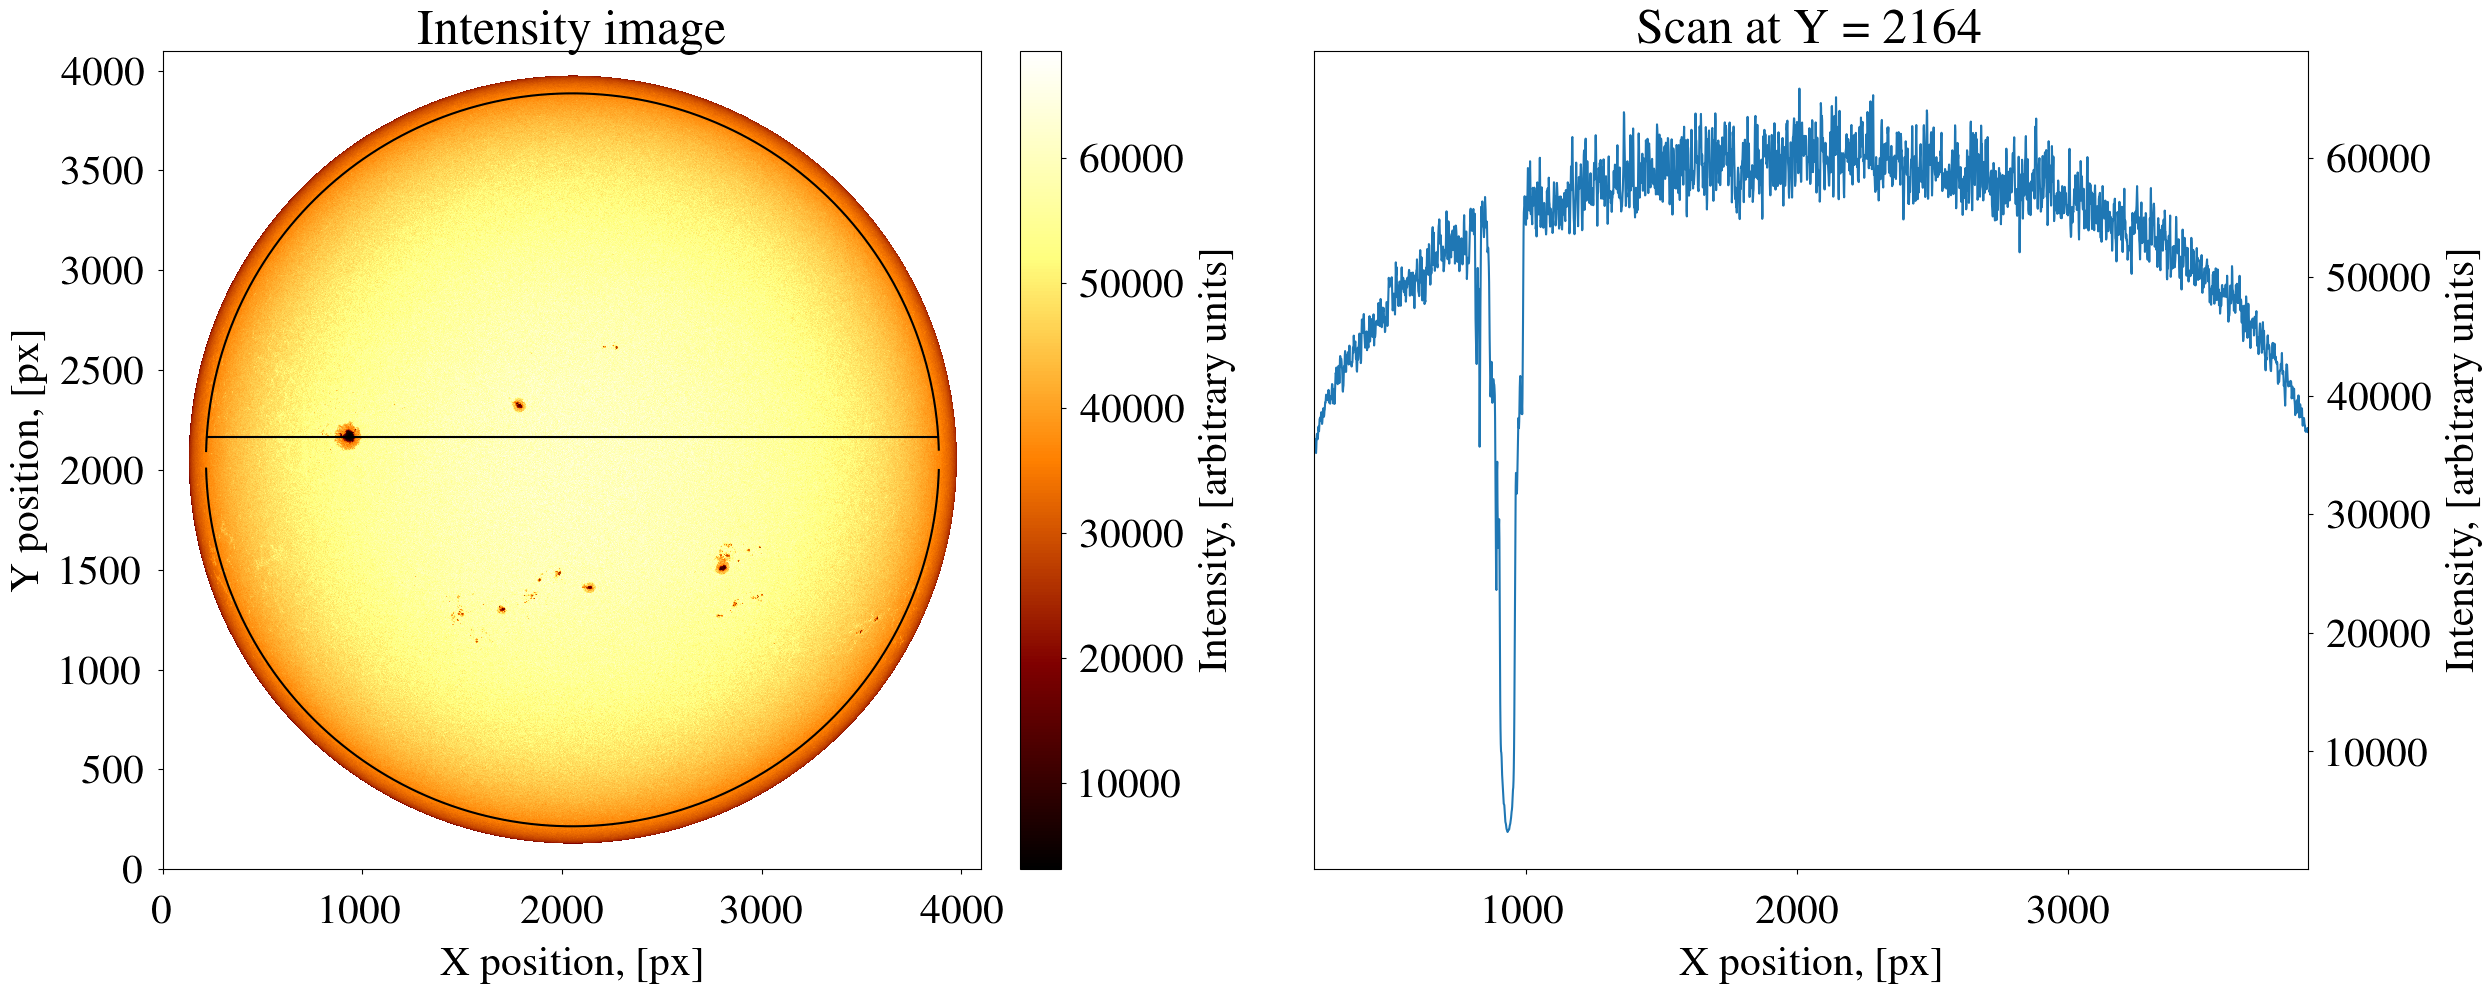
\includegraphics[scale=0.303]{int_scan_orig}
\caption[]{Scan of the intensity image (see left panel of Fig.~\ref{fig:sdo_img}) within $r = 0.953R_\odot$ circumference
           at the $Y$-position of the biggest sun-spot.}
\label{fig:int_scan}
\end{figure*}
\begin{figure*}[h!]
\centering
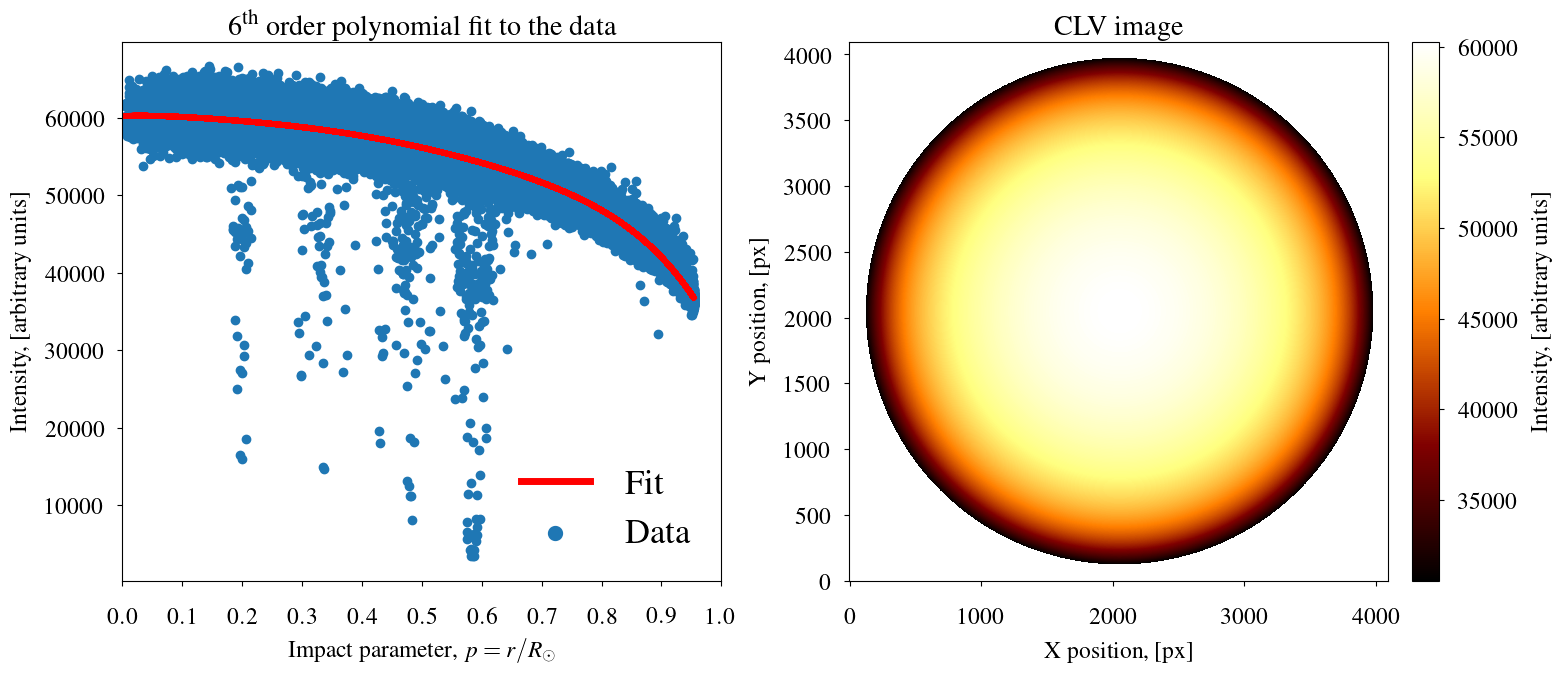
\includegraphics[scale = 0.483]{clv_img}
\caption[]{\textbf{Left panel:} the cloud of data points in the intensity image 
           in the left panel of Fig.~\ref{fig:sdo_img} as a function of the impact parameter
           and the $6^\mathrm{th}$ order polynomial fit to this cloud.
           \textbf{Right panel:} the corresponding CLV image constructed from the fit.}
\label{fig:clv_img}
\end{figure*}
It is seen from Fig.~\ref{fig:int_scan} that the background intensity decreases 
as the distance from the disk center increases.
This decrease is called Center-to-Limb Variation (CLV) or limb-darkening.
In the solar atmosphere the radiation at 6137 \AA\ originates below the temperature minimum.
When we look at the regions of the solar disk closer to the limb we see this radiation coming 
from higher layers (see Fig.~\ref{fig:clv_eff}), but still from somewhere below the temperature minimum.
Therefore, since the temperature at the formation height (see Sect.~\ref{sect:eba}) of radiation is lower as we move towards the disk limb
the emerging radiation undergoes the corresponding decrease in intensity.
\begin{figure*}[h!]
\centering
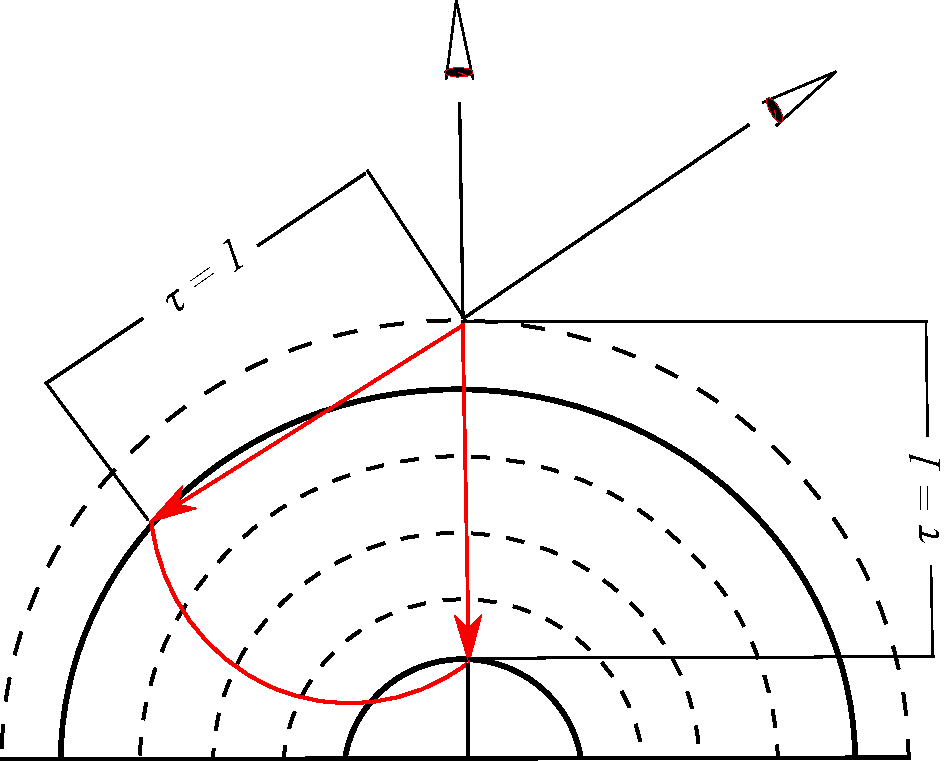
\includegraphics[scale = 0.865]{clv_eff}
\caption[]{The schematic representation of the CLV-effect.
           An observer always sees radiation forming at the layer with $\tau = 1$ 
           ($\tau$ is the optical depth, see Appendix D for details).
           When the line of sight differs from the direction perpendicular to the solar disk the
           $\tau = 1$ level is reached at a higher level.}
\label{fig:clv_eff}
\end{figure*}

The CLV effect has to be removed in order for the analysis of the intensity image to be facilitated,
or in other words the intensity image has to be normalized with respect to the CLV background.
To do this we first map the $(x, y)$ dependence of the image intensity into its radial dependence:
\begin{equation}
I(x, y) \rightarrow I(r(x, y)),
\end{equation}
where
\begin{equation}
r(x, y) = \sqrt{(x - x_0)^2 + (y - y_0)^2}.
\end{equation}
This mapping gives the cloud of points shown in the left panel of Fig.~\ref{fig:clv_img},
for which we then find the best-fit 6$^\mathrm{th}$ order polynomial:
\begin{verbatim}
    >>> import numpy as np

    >>> import numpy.polynomial.polynomial as poly

    >>> c = poly.polyfit(r, Ir, 6)
\end{verbatim}
where $c$ is the array of polynomial coefficients.
Now, we construct the CLV image (see the right panel of Fig.~\ref{fig:clv_img}):
\begin{equation}
I_\mathrm{clv}(x, y) = I_\mathrm{fit}(r(x, y)) = \sum\limits_{i = 0}^6c_ir^i(x, y).
\end{equation}
The procedure building a CLV image for a given intensity image is given in Appendix A.

When we have built the CLV image we might want to save it in binary (\texttt{.npz}) format in order for it
to be faster accessible at the following stages of the analysis (for example, plotting).
The procedure for saving any array structure in \texttt{python} in binary format is as follows:
\begin{verbatim}
    >>> import numpy as np

    >>> np.savez(filename, array1 = array1, array2 = array2, array3 = array3)
 
    >>> arrays = np.load(filename + '.npz') # pay heed to the "+ '.npz'" part
                                           # variable "arrays" works as a dictionary
 
    >>> array1 = arrays['array1']
    >>> array2 = arrays['array2']
    >>> array3 = arrays['array3']

\end{verbatim}

\subsection{Image normalization and signal/noise threshold}
Having calculated the CLV image, we obtain the normalized intensity image as:
\begin{equation}
I_n(x, y) = \frac{I(x, y)}{I_\mathrm{clv}(x, y)},
\end{equation}
where $I(x, y)$ is the original image (see the left panel of Fig.~\ref{fig:int_scan}) and $I_\mathrm{clv}(x, y)$ is the CLV image
(see the right panel of Fig.~\ref{fig:clv_img}). The normalized image is shown in the left panel of Fig.~\ref{fig:int_scan_norm}.
\begin{figure*}[h!]
\centering
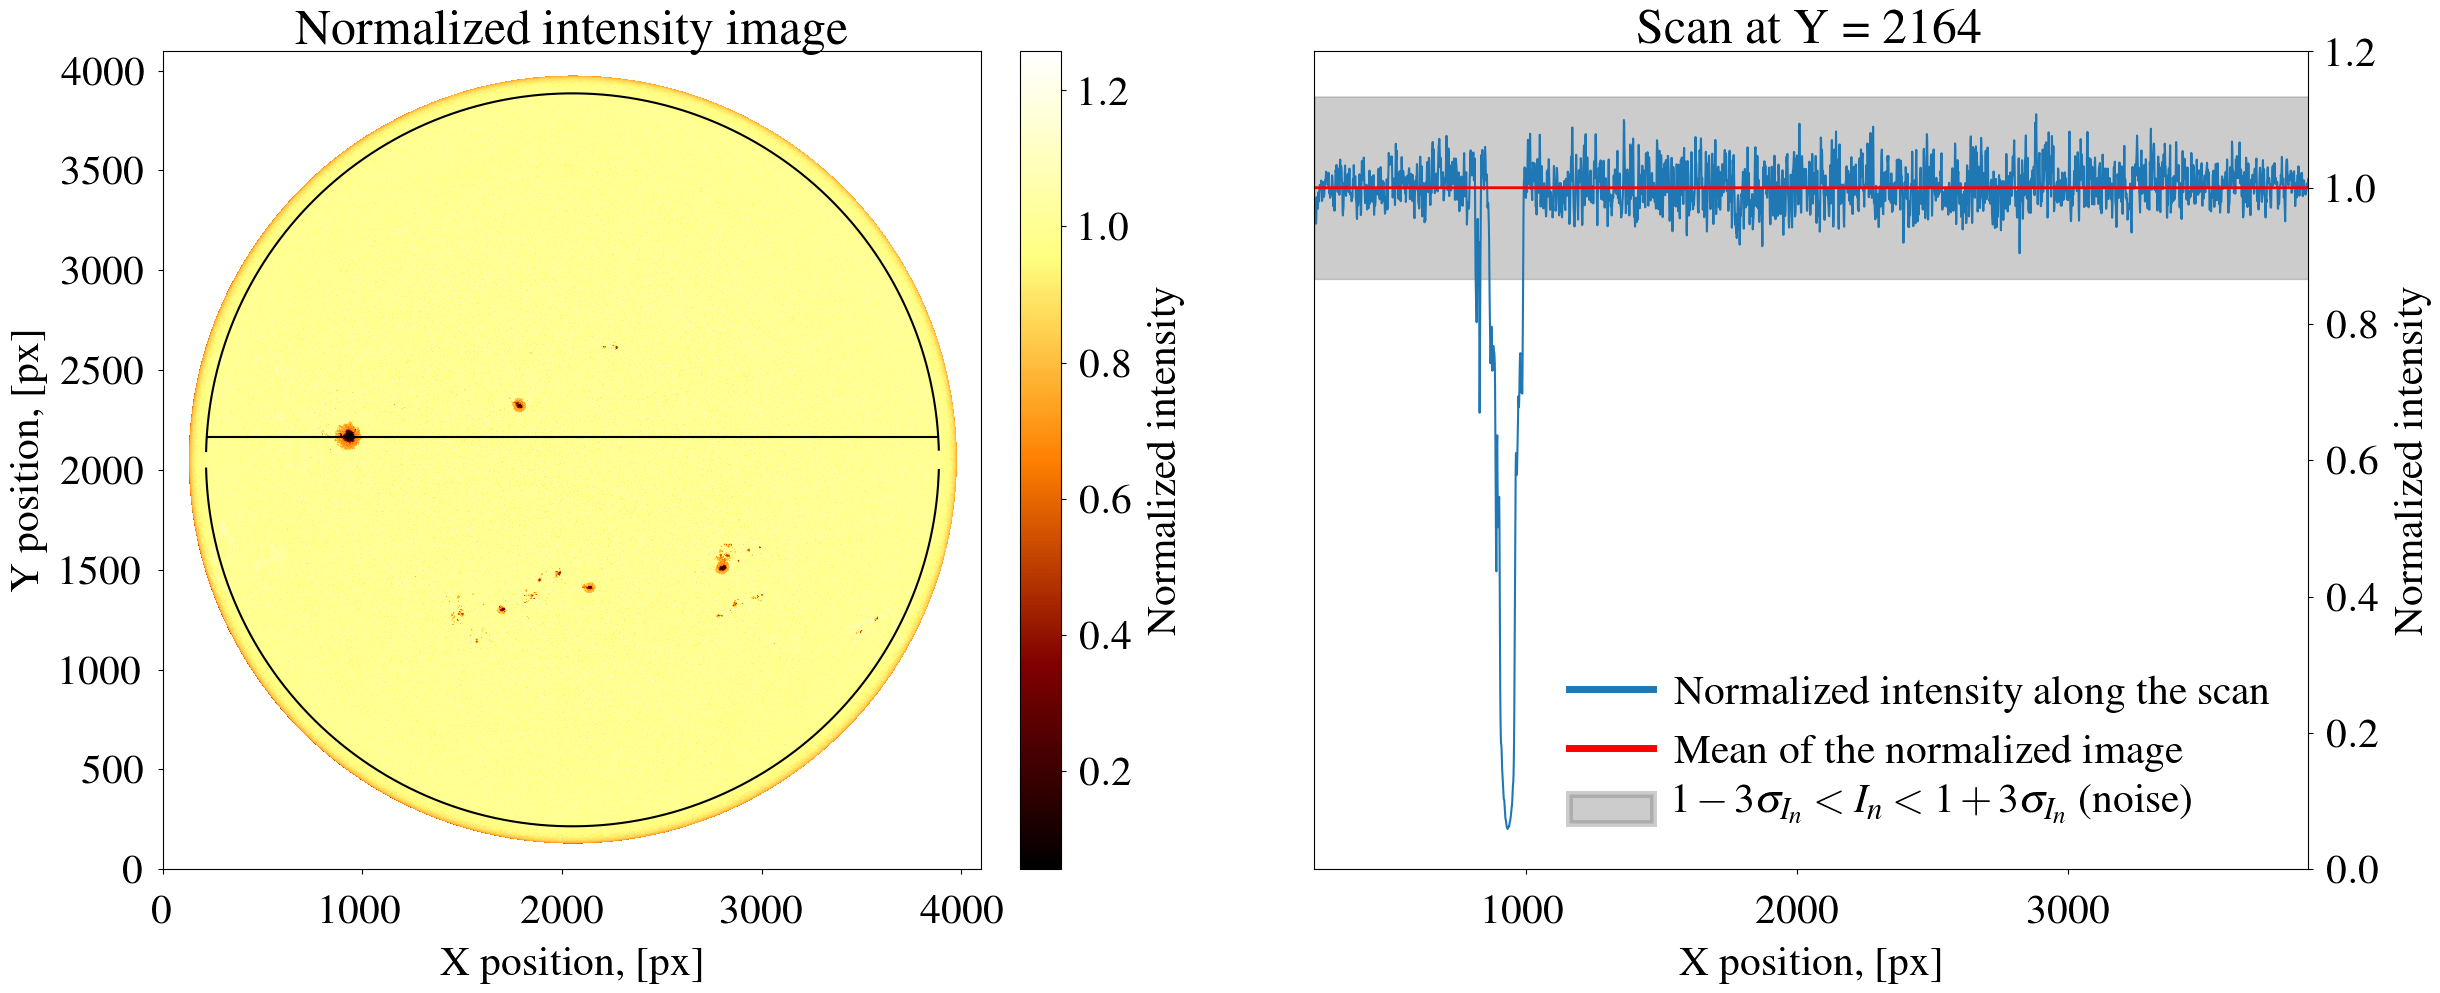
\includegraphics[scale = 0.307]{int_scan_norm}
\caption[]{\textbf{Left panel:} Normalized intensity image 
           (i.e. that in the left panel of Fig.~\ref{fig:int_scan} divided by the CLV image in the right panel of Fig.~\ref{fig:clv_img})
           \textbf{Right panel:} scan of the normalized intensity image within $r = 0.953R_\odot$ circumference at the $Y$-position of the biggest sun-spot.}
\label{fig:int_scan_norm}
\end{figure*}

Analogously to the right panel of Fig.~\ref{fig:int_scan} 
the right panel of Fig.~\ref{fig:int_scan_norm} shows the scan of the normalized image at the $Y$-position of the biggest spot.
The red line indicates the mean value of the normalized image.
This mean value should be equal to one if the normalization is done properly.
The way normalization has been done here suffers from the presence of the outliers in the scatter plot in the left 
panel of Fig.~\ref{fig:clv_img}, therefore the mean of the normalized intensity we actually obtain is slightly lower than one (0.9937).
A more consistent approach is required to remedy this. 
We will not get into the details of it here.
However, this might be one of the possible further developments of the project.

Meanwhile, we will force the mean value of the normalized image to be equal to one and calculate the standard deviation of the
normalized image as:
\begin{equation}\label{eq:sigma_I}
\sigma_{I_n} = \sqrt{\frac{1}{N_\odot}\sum\limits_{x, y}\big(I_n(x, y) - 1\big)^2}.
\end{equation}
Here, the summation is carried over all image pixels satisfying the condition:
\begin{equation}\label{rsun_cond}
\sqrt{(x - x_0)^2 + (y - y_0)^2} \le R_\odot
\end{equation}
and $N_\odot$ is the number of these pixels.
We have to take into account that the values of the data
in the original image and CLV image corresponding to the pixels not satisfying condition \eqref{rsun_cond}
are equal to \texttt{NaN}, therefore in the normalized image they are also equal to \texttt{NaN}
and we have to exclude them with the appropriate logical operators:
\begin{verbatim}
    >>> import numpy as np

    >>> sigma = np.sqrt(np.mean((1 - In[np.where(np.logical_not(np.isnan(In)))])**2))
\end{verbatim}
The $r < 0.953R_\odot$ restriction has been ignored here as it does not affect this stage of the analysis.
At the further stages we will come back to this restriction again.

The gray area in the left panel of Fig.~\ref{fig:int_scan_norm} designates the range
\begin{equation}\label{int_noise_cond}
1 - 3\sigma_{I_n} < I_n(x, y) < 1 + 3\sigma_{I_n}.
\end{equation}
All the intensity values in the original image satisfying condition \eqref{int_noise_cond} are considered to contain the noise.
The pixels satisfying the condition
\begin{equation}\label{signal_cond}
1 + 3\sigma_{I_n} < I_n(x, y) < 1 - 3\sigma_{I_n}
\end{equation}
are considered to contain the signal.
The $3\sigma_{I_n}$ value of the threshold ensures that 99.9\% of the noise is excluded.
For the image considered here $\sigma_{I_n} = 0.044623$.
\begin{figure*}[h!]
\centering
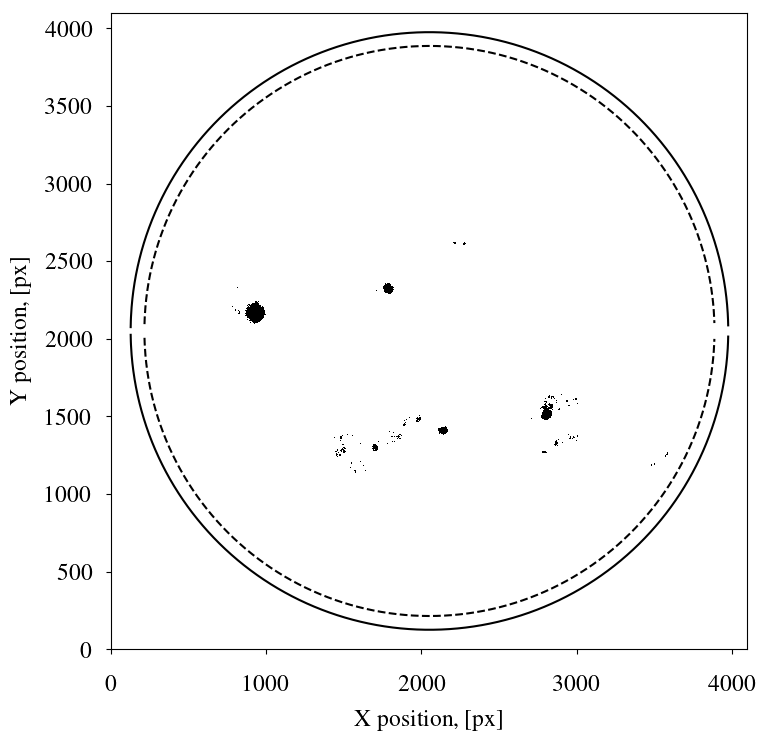
\includegraphics[scale = 0.735]{spt_mask}
\caption[]{Intensity image mask given by Eq.~\eqref{eq:spt_mask}.
           The pixels outside $r = 0.953R_\odot$ circumference (dashed line) have been disregarded.}
\label{fig:spt_mask}
\end{figure*}
\begin{figure*}[h!]
\centering
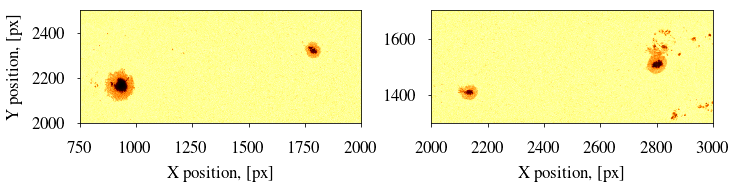
\includegraphics[scale = 0.595]{sdo_int_img_zoom}
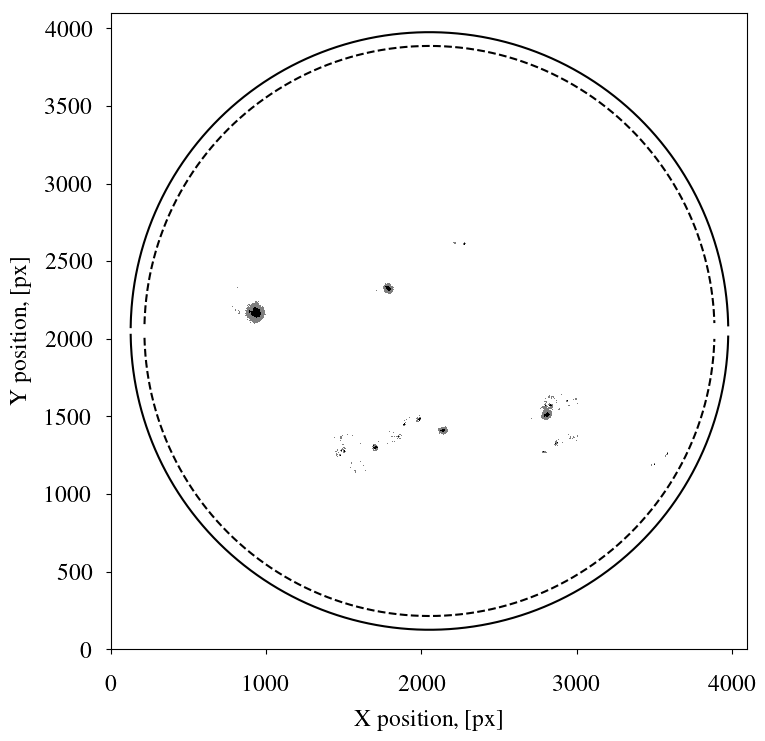
\includegraphics[scale = 0.735]{up_mask}
\caption[]{\textbf{Top panels:} parts of the normalized intensity image (see the left panel of Fig.~\ref{fig:int_scan_norm}) 
           zoomed in to better show the internal division of the spots into umbra and penumbra.
           \textbf{Bottom panel:} intensity image mask given by Eq.~\eqref{eq:up_mask}.
           The pixels outside $r = 0.953R_\odot$ circumference (dashed line) have been disregarded.}
\label{fig:up_mask}
\end{figure*}

\subsection{Intensity image mask}
Having set the signal criterion we can now build the intensity image mask:
\begin{equation}\label{eq:spt_mask}
M_I(x, y) =
\begin{cases}
1,\quad \text{if } I_n(x, y) < 1 - 3\sigma_{I_n}\text{ (signal)}\\
0,\quad \text{otherwise (noise)}.
\end{cases} 
\end{equation}
The mask is concerned only with the intensity signal below $1 - 3\sigma_{I_n}$ level because
our ultimate purpose is the identification of sun-spots which as we know are dark.

Fig.~\ref{fig:spt_mask} shows the intensity mask build from the image in the left panel of Fig.~\ref{fig:sdo_img}
according to Eq.~\eqref{eq:spt_mask}.
As we can see the size of the identified objects varies.
Only the biggest ones are actually spots.
The smaller ones are the so-called pores, which we will not study here.

As can be seen from the top panels of Fig.~\ref{fig:up_mask} the spots are composed of two parts.
The outer brighter part is called penumbra and the inner darker one is called umbra.
The drop of intensity in the spot is caused by the local suppression of convection by the spot's magnetic field.
Since the main mechanism of energy transport below the solar photosphere
\footnote{photosphere, in turn, is the region in the solar atmosphere below the local minimum of its temperature distribution,
this is the region where the radiation at 6173 \AA\ comes from}
is convection this suppression entails the lower temperature in the spot with respect to its surroundings.
In penumbral parts of the spot some forms of magneto-convection maintain their higher temperature with respect to umbra.
The $1 - 3\sigma_{I_n}$ threshold set above corresponds to the outer border of penumbra in the intensity image.
The transition from penumbra to umbra occurs at about $10\sigma_{I_n}$ level.

Having that in mind we now build the intensity image mask taking into account the internal division of spots into
umbra and penumbra:
\begin{equation}\label{eq:up_mask}
M_I^\mathrm{pu}(x, y) =
\begin{cases}
1,  \quad\text{      \ if \ \ \ \ \ \ \ \ \ \ \ \ \ \ \ \ \ }                      I_n(x, y) < 1 - 10\sigma_{I_n}\text{ (umbra signal)}\\
0.5,\quad \text{if } 1 - 10\sigma_{I_n} < I_n(x, y) < 1 - 3\sigma_{I_n}\text{ (penumbra and other signal)}\\
0,  \quad \text{     \ otherwise (noise)}.
\end{cases} 
\end{equation}
The result is shown in the bottom panel of Fig.~\ref{fig:up_mask}.
The procedure for building the intensity masks according to Eqs.~\eqref{eq:spt_mask} and \eqref{eq:up_mask} is given in Appendix B.

\section{Magnetograms}
\subsection{Flux tubes}\label{sect:ftubes}
In terms of spots and faculae identification, finding pixels with magnetic signal
is complementary to finding the dark pixels,
since what is magnetic and dark enough is a spot-like object and what is magnetic and not dark is a facula.
This, in turn, is because topologically spots and faculae are the same.
Roughly, they can be represented as so-called magnetic flux tubes.
Fig.~\ref{fig:fluxtube} shows a sketch of the vertical cross-section of a magnetic flux tube.
The difference between spot and facula is mainly in the radius of its horizontal cross-section.
\begin{figure*}[h!]
\centering
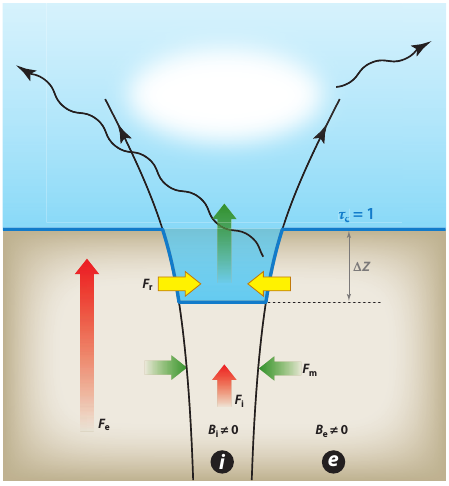
\includegraphics[scale = 0.735]{fluxtube}
\caption[]{Adopted from \cite{solanki2013}. Sketch of the vertical cross section through a magnetic flux tube.
           The red arrows show the vertical convective and radiative energy transport
           inside the flux tube (designated with $i$) and in the external medium (designated with $e$).
           The yellow arrows indicate the horizontal radiative energy flow into the flux tube.
           The rest of the designations are not important.
           }
\label{fig:fluxtube}
\end{figure*}

As has been mentioned above, the convection in a spot is suppressed by the magnetic field.
It is also suppressed in a facular flux tube, but because the latter has a smaller radius
the loss of heat resulting from the suppression of convection is compensated by the radiative
heating coming from the hotter external medium through the walls of the flux tube.
As the radius of the flux tube increases the amount of matter that has to be heated up grows as $\sim R^2$ and
the heat flux into the tube grows as $\sim R$.
Therefore, the radiative inflow through the walls is insufficient to re-heat the matter inside a large flux tube
and it remains cold and dark and is seen as a spot.

\subsection{Finding the signal pixels}
We now proceed to identifying the pixels containing magnetic signal.
Analogously to Fig.~\ref{fig:int_scan}, the magnetogram scan is shown in Fig.~\ref{fig:mag_scan},
in which the values of magnetic field represent the line-of-sight (LOS) component of magnetic field $B_\mu$.
\begin{figure*}[h!]
\centering
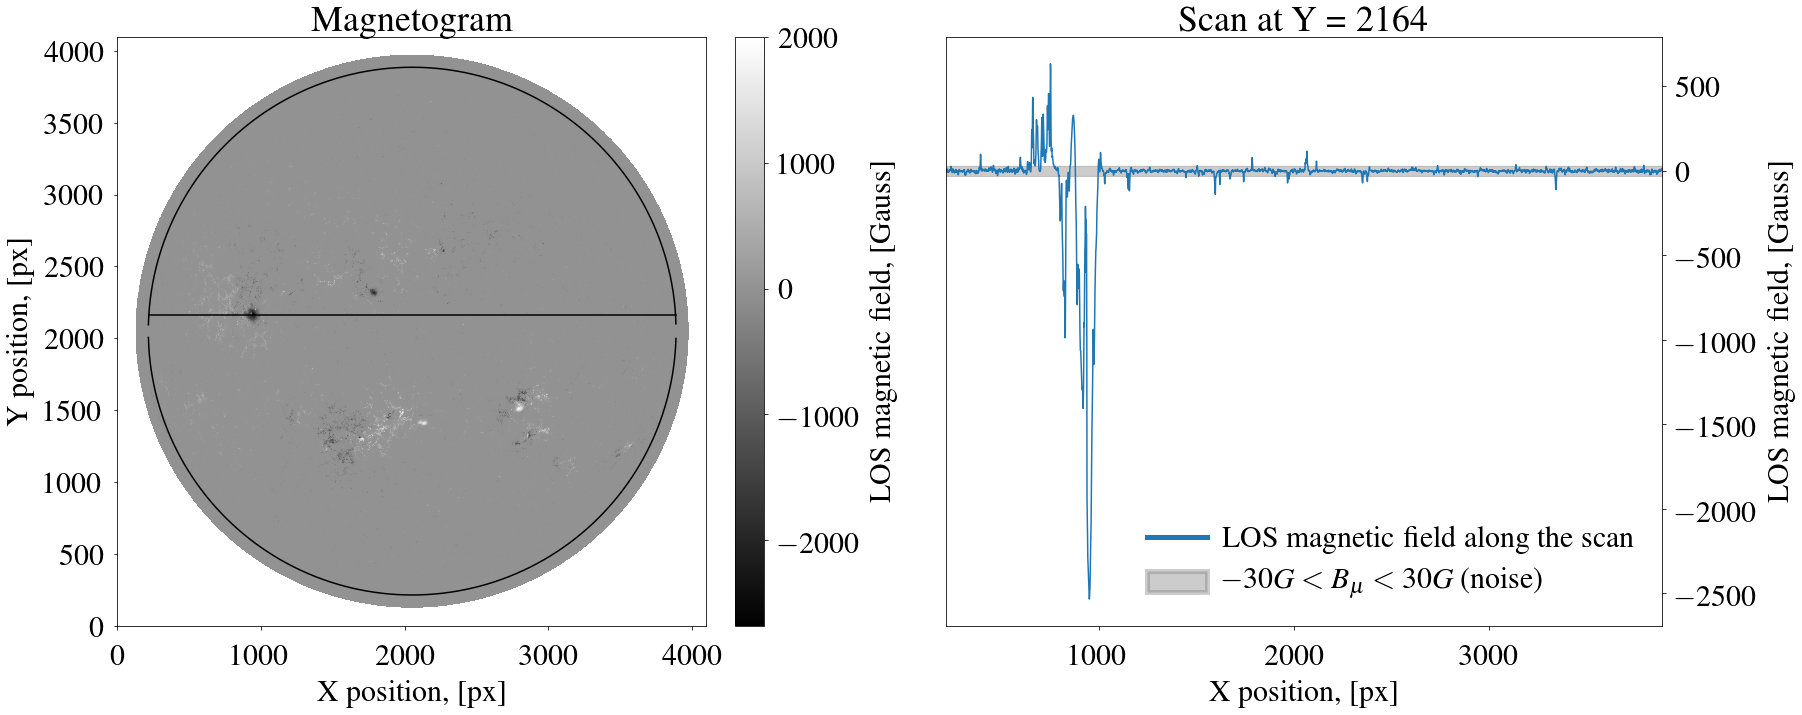
\includegraphics[scale=0.302]{mag_scan}
\caption[]{Magnetogram scan (see the right panel of Fig.~\ref{fig:sdo_img}) within $r = 0.953R_\odot$ circumference
           at the $Y$-position of the biggest sun-spot.}
\label{fig:mag_scan}
\end{figure*}
The LOS component is denoted with the $\mu$ subscript, which is the standard designation for the cosine of
observational angle $\theta$ in solar physics.
This angle is formed by the intersection of LOS corresponding to a certain
position on the solar disk and the local normal to the solar surface (see Fig.~\ref{fig:mu}).
Its cosine is used in solar physics as a measure of radial distance from the solar disk center.
Alternatively, the impact parameter $p$ can be used (see Fig.~\ref{fig:clv_img}, left panel).
Assuming that the local magnetic field is predominantly perpendicular to the
solar surface the relationship between LOS magnetic field $B_\mu$ and
the actual magnetic field can be expressed in terms of $\mu$ (see Fig.~\ref{fig:mu}).
Below we will discuss when this assumption breaks down.
\begin{figure*}[h!]
\centering
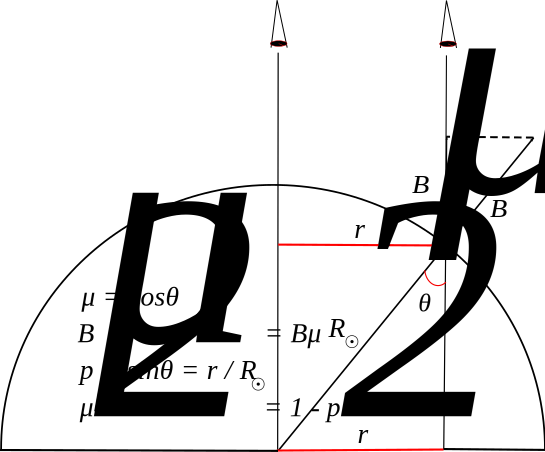
\includegraphics[scale = 0.865]{mu}
\caption[]{Geometry of the observational angle and impact parameter.
           Lines of sight corresponding to different positions on the solar disk
           can be considered parallel, because the observer is far away from the Sun.
           The constraint $r < 0.953R_\odot$ or equivalently $p < 0.953$ introduced in the beginning
           corresponds to $\mu > 0.3$.
           }
\label{fig:mu}
\end{figure*}

The principle of magnetic signal identification is the same as for the intensity images,
except that no normalization has to be performed.
However, in the case of magnetograms, proper calculation of $\sigma_{B_\mu}$ is quite complicated.
We will not get into the details of it here and adopt the value of $\sigma_{B_\mu} = 10G$ for the noise level
(the references to this number will be given a bit later).
The mean magnetic signal is zero as is seen from the right panel of Fig.~\ref{fig:mag_scan}.
Hence, the magnetic mask is given by:
\begin{equation}\label{eq:mag_mask}
M_B(x, y) =
\begin{cases}
1,\quad \text{if } |B_\mu(x, y)| > 3\sigma_{B_\mu} = 30G\text{ (signal)}\\
0,\quad \text{otherwise (noise)}.
\end{cases}
\end{equation}
A procedure building the magnetic mask is given in Appendix B.
In accordance with the discussion in Sect.~\ref{sect:ftubes} the facular mask is calculated as:
\begin{equation}\label{eq:fac_mask}
M_F(x, y) = M_B(x, y) - M_I(x, y).
\end{equation}

The magnetic and facular masks for the images in Fig.~\ref{fig:sdo_img} are shown in Fig.~\ref{fig:mag_fac_mask}
from which we can see the morphological difference between the spot and facular coverages of the solar disk.
Faculae, being much smaller than spots (see Sect~\ref{sect:ftubes}), can cover an area on the 
solar disk which is smaller than the area of one pixel at the disk center
\footnote{the area covered by one pixel depends on $\mu$ because of the projection effect}.
They group together and form the facular structures seen in the right panel of Fig.~\ref{fig:mag_fac_mask}.
In that sense (as opposed to the topological sense, discussed in Sect.~\ref{sect:ftubes})
faculae are different from spots because the latter represent singular spatially resolved objects and the former ---
a conglomeration of (mostly) spatially unresolved objects.

The magnetic field lines in a flux tube diverge.
The horizontal component of the magnetic field grows with
the radial distance from the center of the horizontal cross-section of the flux tube.
In the penumbral parts the field becomes more and more horizontal (see Fig.~\ref{fig:3D_spot}).
That is why we see the $-1$ values in the facular mask.
These values correspond to the outer parts of some spots (i.e. penumbral) 
where the magnetogram values are the actual signal, but
because the LOS component of the field is so low they turned out to be below the 30G LOS magnetic
field threshold (see Eq.~\ref{eq:mag_mask}) and were counted as noise.
Therefore
\begin{equation}
\mbox{if } M_F(x, y) = -1 \Rightarrow M_F(x, y)\equiv 0.
\end{equation}
\begin{figure*}[h!]
\centering
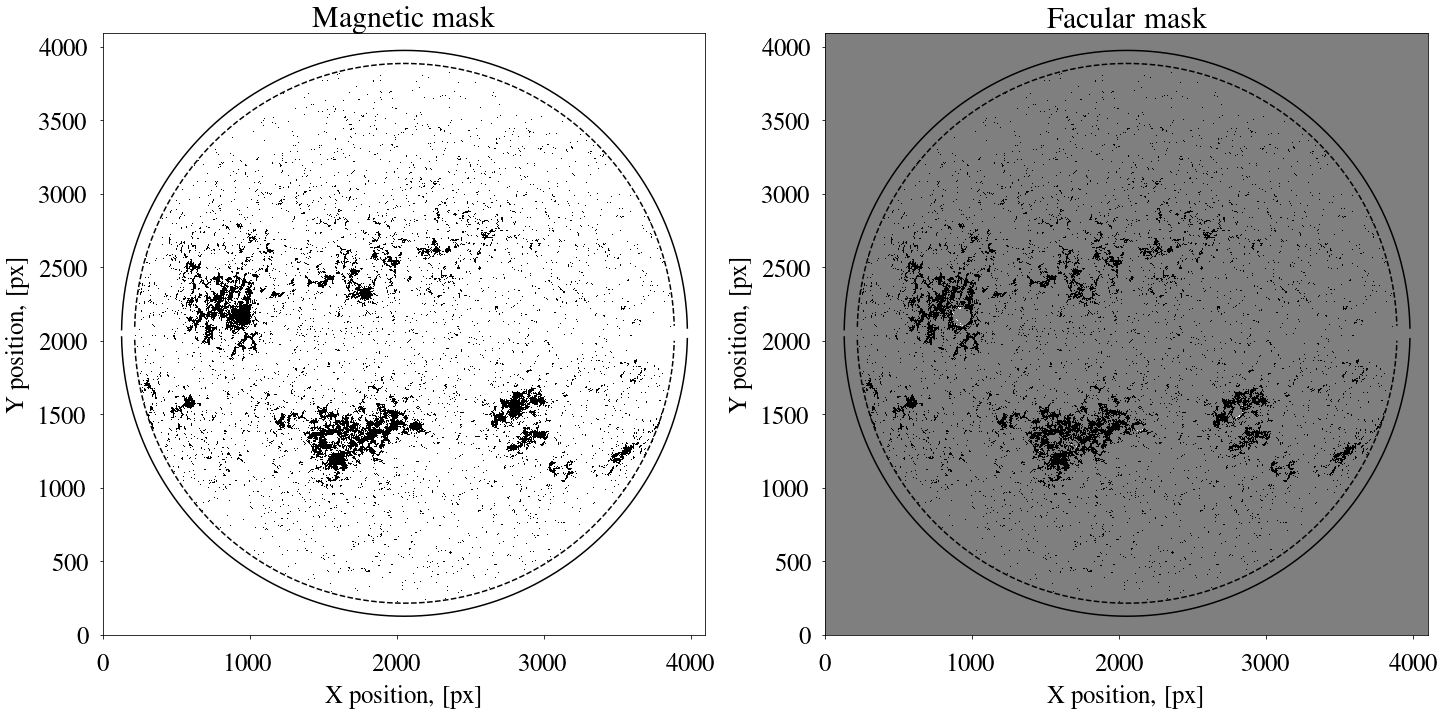
\includegraphics[scale=0.375]{mag_fac_mask}
\caption[]{Magnetic and facular masks for the images in Fig.~\ref{fig:sdo_img} built
           according to Eqs.~\eqref{eq:spt_mask}, \eqref{eq:mag_mask} and \eqref{eq:fac_mask}.
           Color correspondence in the left panel:  white is 0, black is 1.
           Color correspondence in the right panel: white is $-1$, gray is 0, black is 1.
           The pixels outside $r = 0.953R_\odot$ circumference have been disregarded.}
\label{fig:mag_fac_mask}
\end{figure*}
\begin{figure*}[h!]
\centering
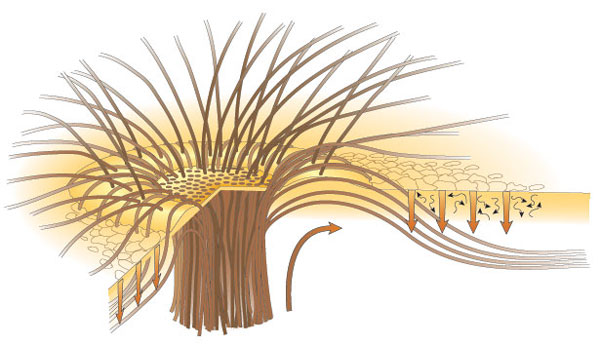
\includegraphics[scale=0.575]{3D_spot}
\caption[]{Adopted from \cite{thomas2002}. Sketch of 3D sun-spot magnetic field structure showing almost horizontal
           magnetic field in the penumbral regions of a sun-spot.}
\label{fig:3D_spot}
\end{figure*}

\section{Facular and umbral magnetic fields and spot sizes}
Having the intensity and magnetic masks we can now look at the typical facular and spot magnetic fields and also
calculate the typical sizes of sun-spots.
Because of the predominantly horizontal alignment of the magnetic field in the penumbra (see Fig.~\ref{fig:3D_spot}),
the determination of penumbral magnetic fields is obstructed.
When penumbra is seen at the limb its magnetic field is aligned with LOS,
otherwise it is predominantly out of alignment and there is no simple way to
obtain the actual magnetic field from the penumbral LOS magnetic field component.
Hence, we will only concern ourselves with facular and umbral magnetic fields which are predominantly perpendicular
to the local solar surface (as was explained above) and therefore the actual magnetic field can be obtained from the
LOS magnetic field by means of the observational angle correction (see Fig.~\ref{fig:mu}).
The determination of the sizes of faculae is, in turn, obstructed by their smallness and conglomeration.
\begin{figure*}[h!]
\centering
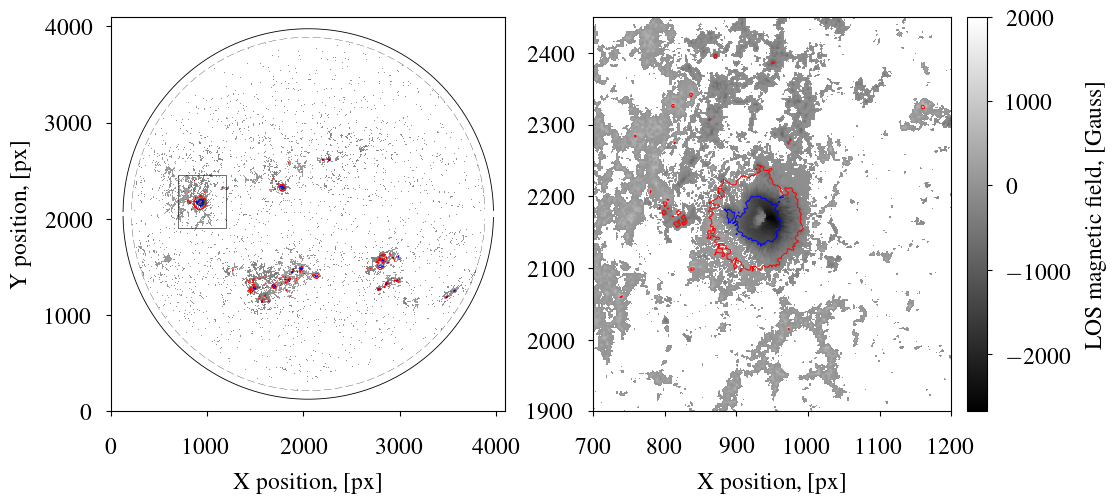
\includegraphics[scale=0.685]{spt_cnts}
\caption[]{\textbf{Left panel:} Magnetic mask built according to Eq.~\eqref{eq:mag_mask_prime}.
           The umbral and penumbral contours are shown in blue and red respectively.
           The pixels outside $r = 0.953R_\odot$ circumference have been disregarded.
           \textbf{Right panel:} Zoom-in of the box in the left panel.}
\label{fig:spt_cnts}
\end{figure*}

Fig.~\ref{fig:spt_cnts} shows the magnetic mask
\begin{equation}\label{eq:mag_mask_prime}
M_B'(x, y) =
\begin{cases}
B_\mu(x, y),\quad \text{if } |B_\mu(x, y)| > 3\sigma_{B_\mu} = 30G\\
\mathrm{NaN},\quad \text{otherwise},
\end{cases}
\end{equation}
with the values of LOS magnetic field from the original magnetogram along with the penumbral and umbral contours.
The typical values of facular and umbral magnetic fields can be obtained by making a scatter plot of all magnetic
field values outside the red contours and inside the blue contours, respectively, as a function of radius
(or any other measure of radial distance) or $X$-position or $Y$-position or pixel number
(though in the last case it would not be a scatter plot).
The observational angle correction of magnetic field (see Fig.~\ref{fig:mu}) has to be implemented before the plotting
\footnote{the observational angle has to be calculated for each pixel of the magnetogram}.

The typical spot sizes can be obtained by labeling spots in Fig.~\ref{fig:spt_mask}:
\begin{verbatim}
>>> from scipy.ndimage import measurements

>>> labeled_spot_mask, number_of_spots  = measurements.label(original_spot_smask)
\end{verbatim}
and summing the areas of individual spot pixels, having implemented the observational angle correction to the said areas
\footnote{the correction of pixel area is analogous to the magnetic field correction}.

Both tasks can be quite easily performed using the intensity, magnetogram and facular masks in
combination with applying the \texttt{numpy.where} function.
In some cases \texttt{numpy.logical\_not} and \texttt{numpy.isnan} functions might be needed.
The procedure for plotting the umbral and penumbral contours (see Fig.~\ref{fig:spt_cnts}) is given in Appendix C.

\clearpage
\section{Appendix A: procedure for building the CLV image}
\small
\begin{verbatim}
1   import numpy as np
2
3   import numpy.polynomial.polynomial as poly
4
5   from tqdm import tqdm # this is just a package for making nice progress bars
6
7   def clv(int_img, x0, y0, r, rsun): # r = 0.953 * rsun
8 
9       rad = its = np.array([])       # rad and its are 1D-arrays here
10 
11      y1 = int(np.ceil(y0 - r))
12      y2 = int(np.ceil(y0 + r))
13 
14      for ys in tqdm(range(y1, y2), desc = 'Building I(r)'):
15 
16          if ys % 2 != 0: continue
17 
18          x = np.arange(4096)
19
20          x1 = x0 - np.sqrt(r**2 - (ys - y0)**2)
21          x2 = x0 + np.sqrt(r**2 - (ys - y0)**2)
22
23          idx_scan = np.where((x >= x1) & (x <= x2) & (x % 2 == 0))
24
25          xs = x[idx_scan]
26
27          rs = np.sqrt((xs - x0)**2 + (ys - y0)**2)
28
29          ints = int_img[ys, idx_scan[0]]
30 
31          its = np.concatenate((its, ints))
32 
33          rad = np.concatenate((rad, rs))
34 
35      c = poly.polyfit(rad, its, 6)
36 
37      ld_img = np.zeros((4096, 4096))
38 
39      y1 = int(np.ceil(y0 - rsun))
40      y2 = int(np.floor(y0 + rsun))
41 
42      for ys in tqdm(range(y1, y2), desc = 'Building CLV image'):
43
44          x = np.arange(4096)
45 
46          x1 = x0 - np.sqrt(rsun**2 - (ys - y0)**2)
47          x2 = x0 + np.sqrt(rsun**2 - (ys - y0)**2)
48 
49          idx_scan = np.where((x >= x1) & (x <= x2))
50 
51          xs = x[idx_scan]
52 
53          rs = np.sqrt((xs - x0)**2 + (ys - y0)**2)
54 
55          ld_img[ys, idx_scan[0]] = poly.polyval(rs, c)
56 
57      return ld_img
\end{verbatim}

\clearpage
\section{Appendix B: procedure for building the spot/umbra/penumbra/magnetic masks}
\small
\begin{verbatim}
1  import numpy as np
2
3  from tqdm import tqdm # this is just a package for making nice progress bars
4
5  def rad(x0, y0):
6 
7      rad = np.zeros((4096, 4096))
8 
9      for x in tqdm(range(4096), desc = 'Calculating r(x, y)'):
10 
11         for y in range(4096):
12 
13             rad[y, x] = (x - x0)**2 + (y - y0)**2
14 
15     rad = np.sqrt(rad)
16 
17     return rad
18 
19 def intensity_mask(I, r, rad): # r = 0.953 * rsun # rad is calculated as a 2D-array above
20 
21     sigma = np.sqrt(np.mean((1 - I[np.where(np.logical_not(np.isnan(I)))])**2))
22 
23     I[np.where(np.isnan(I))] = 0.0
24 
25     Ip = 1 - 3 * sigma
26
27     Iu = 1 - 10 * sigma
28 
29     mask_s = np.zeros((4096, 4096))
30     mask_u = np.zeros((4096, 4096))
31     mask_p = np.zeros((4096, 4096))
32 
33     mask_s[np.where((rad <= r) & (I <= Ip) & (I != 0.0))] = 1.0
34 
35     mask_u[np.where((rad <= r) & (I <= Iu) & (I != 0.0))] = 1.0
36
37     mask_p[np.where((rad <= r) & (I > Iu) & (I <= Ip) & (I != 0.0))] = 0.5
38 
39     return mask_s, mask_u, mask_p
40
41 def magnetic_mask(B, r, rad): # r = 0.953 * rsun # rad is calculated as a 2D-array above
42 
43     B[np.where(np.isnan(B))] = 0.0
44 
45     sigma = 10.0
46 
47     mask = np.zeros((4096, 4096))
48 
49     mask[np.where((rad <= r) & ((B <= -3.0 * sigma) | (B >= 3.0 * sigma)) & (B != 0.0))] = 1.0
50 
51     return mask
\end{verbatim}

\clearpage
\section{Appendix C: procedure for deriving and plotting umbral and penumbral contours}
\small
\begin{verbatim}
1  import numpy as np
2  
3  import cv2
4
5  def get_cnt_coord(cnt):
6
7      x = np.array([])
8      y = np.array([])
9
10     for elem in cnt:
11
12         x = np.concatenate((x, [elem[0][0]]))
13         y = np.concatenate((y, [elem[0][1]]))
14
15     first_elem = cnt[0]
16
17     x = np.concatenate((x, [first_elem[0][0]]))
18     y = np.concatenate((y, [first_elem[0][1]]))
19
20     return x, y
21
22 shapes_p = cv2.inRange(mask_p, 0.4, 0.6)
23 shapes_u = cv2.inRange(mask_u, 0.9, 1.1)
24
25 # w1 and w2 stand for "whatever1" and "whatever2", we do not need these outputs
26 # get the info on the second output to understand how the function get_cnt_coord works
27
28 w1, cnts_p, w2 = cv2.findContours(shapes_p.copy(), cv2.RETR_EXTERNAL, cv2.CHAIN_APPROX_SIMPLE)
29 w1, cnts_u, w2 = cv2.findContours(shapes_u.copy(), cv2.RETR_EXTERNAL, cv2.CHAIN_APPROX_SIMPLE)
30
31 # ... some stuff here ...
32
33 for cnt in cnts_p:
34
35     x_cnt, y_cnt = get_cnt_coord(cnt)
36
37     plt.plot(x_cnt, y_cnt, '-', color = 'r')
38
39 for cnt in cnts_u:
40
41     x_cnt, y_cnt = get_cnt_coord(cnt)
42
43     plt.plot(x_cnt, y_cnt, '-', color = 'b')
44
45 # ... some more stuff here ...
\end{verbatim}

\clearpage
\section{Appendix D: Radiative transfer equation}\label{sect:rte}
\subsection{Derivation of the general form}\label{sect:dgf}
The main quantity of interest in the theory of radiative transfer is the intensity of radiation.
The intensity is defined as the amount of energy carried by the photons within a frequency interval $d\nu$,
through area $d\sigma$, over time $dt$, within solid angle $d\omega$ around the direction $\mb{n}$:
\begin{equation}\label{eq:int}
dE_\nu(\mb{r}, \mb{n}, t) = I_\nu(\mb{r}, \mb{n}, t) d\sigma dtd\nu d\omega.
\end{equation}
Here, $\mb{r}$ is the radius-vector of the point in space where the intensity is measured.

The transport of radiation through a medium is mathematically formulated with the equation of radiative transfer which
describes the evolution of intensity along direction $\mb{n}$.
The physical meaning of this equation is conservation of energy, i.e. that the intensity
along the ray $\mb{n}$ does not change unless photons are added into the beam or taken out of it.
To write the conservation of energy we need the quantities characterizing the loss and gain of photons in the beam.

The gain of energy of frequency $\nu$ is quantified with the emissivity $\eta_\nu(\mb{r}, \mb{n}, t)$
which is the amount of energy $dE_\nu$ added by the volume $dV$ into the beam of photons with frequencies within $d\nu$
and directions within $d\omega$ around vector $\mb{n}$ per time $dt$:
\begin{equation}\label{eq:emis}
dE^+_\nu(\mb{r}, \mb{n}, t) = \eta_\nu(\mb{r}, \mb{n}, t)dVdtd\nu d\omega.
\end{equation}

The loss of energy is characterized by the absorption coefficient (or opacity) $\chi_\nu$
defined so that the fraction of intensity subtracted from the beam within the length interval $ds$
along the ray $\mb{n}$ is $\chi_\nu ds$.
Therefore the corresponding decrease of the beam energy is
\begin{equation}\label{eq:abs}
dE^-_\nu(\mb{r}, \mb{n}, t) = \chi_\nu I_\nu(\mb{r}, \mb{n}, t)dsd\sigma dtd\nu d\omega.
\end{equation}

We can now write the equation of radiative transfer using simple energy conservation considerations \cite{mihalas1978, rutten2003}.
The amount by which the energy of the beam at frequency $\nu$ changes as it passes the length interval $ds$ is:
\begin{subequations}\label{eq:en_change}
\begin{equation}
dE^+_\nu - dE^-_\nu = \big(I_\nu(\mb{r} + \mb{dr}, \mb{n}, t + dt) - I_\nu(\mb{r}, \mb{n}, t)\big)d\sigma dtd\nu d\omega \label{eq:change1}\\
\end{equation}
\begin{equation}
=\big(\eta_\nu(\mb{r}, \mb{n}, t) - \chi_\nu I_\nu(\mb{r}, \mb{n}, t)\big)dsd\sigma dtd\nu d\omega, \label{eq:change2}
\end{equation}
\end{subequations}
where $ds = |d\mb{r}|$ and we took into account that $dV = dsd\sigma$.
In Eq.~\eqref{eq:change1} we used the definition of intensity (Eq.~\ref{eq:int})
and when transitioning from Eq.~\eqref{eq:change1} to Eq.~\eqref{eq:change2} we used the definitions \eqref{eq:emis} and \eqref{eq:abs}.
Taking into account that $dt = ds / c$, where $c$ is the speed of light, we write the difference of intensities as:
\begin{equation}\label{eq:int_der}
I_\nu(\mb{r} + \mb{dr}, \mb{n}, t + dt) - I_\nu(\mb{r}, \mb{n}, t) =
\left(\frac{1}{c}\frac{\partial I_\nu}{\partial t} + \frac{\partial I_\nu}{\partial s}\right)ds =
\left(\frac{1}{c}\frac{\partial I_\nu}{\partial t} + \mb{n}\nabla I_\nu\right)ds.
\end{equation}
Here, we wrote the directional derivative $\partial / \partial s$ along vector $\mb{n}$ in terms of the $\nabla$ operator.
Substituting the derivative \eqref{eq:int_der} into Eq.~\eqref{eq:en_change} we arrive 
at the general form of the equation of radiative transfer:
\begin{equation}\label{eq:rte_app}
\left(\frac{1}{c}\frac{\partial}{\partial t} + \mb{n}\nabla\right)I_\nu(\mb{r}, \mb{n}, t) = \eta_\nu(\mb{r}, \mb{n}, t) -
\chi_\nu(\mb{r}, \mb{n}, t) I_\nu(\mb{r}, \mb{n}, t).
\end{equation}
\subsection{Plain-parallel geometry}\label{sect:ppg}
Let us consider now the simplest geometrical case of a static non-expanding medium that is comprised of plane-parallel slabs.
In each slab the properties of the medium remain the same both in space and time.
We introduce the Cartesian system of coordinates with axis $z$ perpendicular to the slabs, 
along which the properties of the medium change (see Fig.~\ref{fig:ppa}), and the observational angle $\theta$ with respect to axis $z$.
In the Cartesian system of coordinates the directional derivative $\mb{n}\nabla$ is:
\begin{equation}
\mb{n}\nabla = n_x\frac{\partial}{\partial x} + n_y\frac{\partial}{\partial y} + n_z\frac{\partial}{\partial z}.
\end{equation}
In the case of plain-parallel geometry $\partial / \partial x = 0$, $ \partial / \partial y = 0$.
Therefore, taking into account that the medium is static ($\partial / \partial t = 0$),
the radiative transfer equation takes the form:
\begin{equation}\label{eq:rte_pp}
\mu\frac{dI_\nu(z, \mu)}{dz} = \eta_\nu(z) - \chi_\nu(z)I_\nu(z, \mu),
\end{equation}
where $\mu = \cos\theta = n_z$.
Dividing both sides of the last equation by $-\chi_\nu$ and designating $S_\nu = \eta_\nu / \chi_\nu$ we write:
\begin{equation}\label{eq:rte_mus}
\mu\frac{dI_\nu(\tau_\nu, \mu)}{d\tau_\nu} = I_\nu(\tau_\nu, \mu) - S_\nu(\tau_\nu),
\end{equation}
where
\begin{equation}\label{eq:optd}
d\tau_\nu = -\chi_\nu(z)dz
\end{equation}
is increment of the so-called optical depth or length, which is the ``effective distance'' for photons.
The physical meaning of optical depth is that in the process of radiative transfer across a certain distance, 
not the distance itself, but the strength of absorption of the radiation by the medium 
determines how ``hard'' it is for photons to travel across this distance.
It is convenient to measure the optical depth in the direction opposite to that of $z$ axis in Fig.~\ref{fig:ppa}
(hence the minus sign in Eq.~\ref{eq:optd}).
The quantity $S_\nu(\tau_\nu)$ is called the source function.
It describes the influence of the medium on the intensity of the beam.
\begin{figure}
\centering
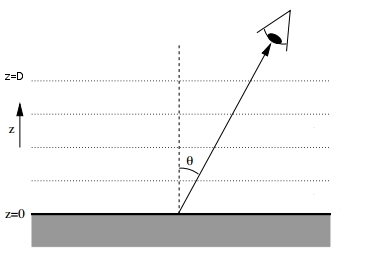
\includegraphics[scale=1.1]{ppa_corr}
\caption[Plane-parallel geometry]{
         Plane-parallel geometry: the simplest case for which the radiative transfer equation can be written.
         The $z$ axis is perpendicular to the parallel slabs of the medium in which its properties remain the same.
         The observer sees radiation coming at angle $\theta$ with respect to axis $z$.
        }
\label{fig:ppa}
\end{figure}

\subsection{Eddington-Barbier approximation}\label{sect:eba}
Eq.~\eqref{eq:rte_mus} can be solved analytically for inward directed intensity ($\mu < 0$)
and outward directed intensity ($\mu > 0$) \cite[p. 17]{rutten2003}:
\begin{equation}\label{eq:fs}
I_\nu(\tau_\nu, \mu) =
\begin{cases}
&-\int\limits_0^{\tau_\nu}S_\nu(t_\nu)\mbox{e}^{-(t_\nu - \tau_\nu) / \mu}dt_\nu / \mu, \quad \mu < 0,\\
&+\int\limits_{\tau_\nu}^\infty S_\nu(t_\nu)\mbox{e}^{-(t_\nu - \tau_\nu) / \mu}dt_\nu / \mu, \quad \mu > 0.
\end{cases}
\end{equation}
Solution given by Eq.~\eqref{eq:fs} is called formal solution, since it expresses the intensity $I_\nu(\tau_\nu, \mu)$ in terms of the
source function $S_\nu(\tau_\nu)$ which is not always known in advance.

According to the formal solution the emergent ($\tau_\nu = 0$) outward intensity as seen by the observer in Fig.~\ref{fig:ppa} is:
\begin{equation}\label{eq:em_int}
I_\nu^+(\tau_\nu = 0, \mu) = \int\limits_0^\infty S_\nu(t_\nu)\mbox{e}^{-t_\nu / \mu}dt_\nu / \mu.
\end{equation}
Substituting the Taylor expansion of the source function
\begin{equation}\label{eq:sfte}
S_\nu(\tau_\nu) = \sum\limits_{n=0}^\infty a_n\tau_\nu^n
\end{equation}
into Eq.~\eqref{eq:em_int} and using the integral representation of the factorial
\begin{equation}
n! = \int\limits_0^\infty x^n\mbox{e}^{-x}dx,
\end{equation}
we obtain the Taylor expansion of the emergent intensity in terms of the cosine of the observational angle $\mu$:
\begin{equation}\label{eq:emite}
I_\nu^+(\tau_\nu = 0, \mu) = \sum\limits_{n=0}^\infty n!a_n\mu^n.
\end{equation}
Comparing Eq.~\eqref{eq:sfte} and Eq.~\eqref{eq:emite} we arrive at the Eddington-Barbier approximation:
\begin{equation}\label{eq:eb_app}
I_\nu^+(\tau_\nu = 0, \mu) \approx S_\nu(\tau_\nu = \mu).
\end{equation}
Hence, the radiation coming in the direction $\mu$ forms at the layer with $\tau_\nu\approx\mu$
($\tau\approx 1$ for the radiation coming along the direction perpendicular to the slabs of the medium).
Thus, the notion of the formation height arises.
The formation height of the radiation observed along the direction $\mu$ is defined as the height of the layer in the medium with $\tau_\nu = \mu$.
Using the definition of optical depth (Eq.~\ref{eq:optd}) we can write the
condition from which the formation height $h_f$, as seen from the direction $\mu$, can be found:
\begin{equation}
\mu = -\int\limits_D^{h_f}\chi_\nu dz,
\end{equation}
where $D$ is the height of the topmost layer of the medium (see Fig.~\ref{fig:ppa}).

\printbibliography

\end{document}
%For estimating the sizes of spots it would be convenient to get rid of the smallest objects in the intensity mask in Fig.~\ref{fig:spt_mask}.
%This can be done by means of smoothing the original intensity image, so that:
%\begin{equation}\label{eq:smh}
%I_s(x, y) = \iint I(x', y')G(x' - x, y' - y)dx'dy',
%\end{equation}
%where
%\begin{equation}
%G(x' - x, y' - y) = G_0\exp\left(-\left\{\frac{(x' - x)^2}{2\sigma_x^2} + \frac{(y' - y)^2}{2\sigma_y^2}\right\}\right)
%\end{equation}
%is the Gaussian filter with $\sigma_x$, $\sigma_y$ being the widths of the Gaussian kernel along 
%$X$ and $Y$ directions and
%\begin{equation}
%\iint G(x' - x, y' - y)dx'dy' = 1.
%\end{equation}
%\begin{verbatim}
%    from scipy.ndimage import filters
%
%    Is = filters.gaussian_filter(I, 10)
%\end{verbatim}
%\begin{figure*}[h!]
%\centering
%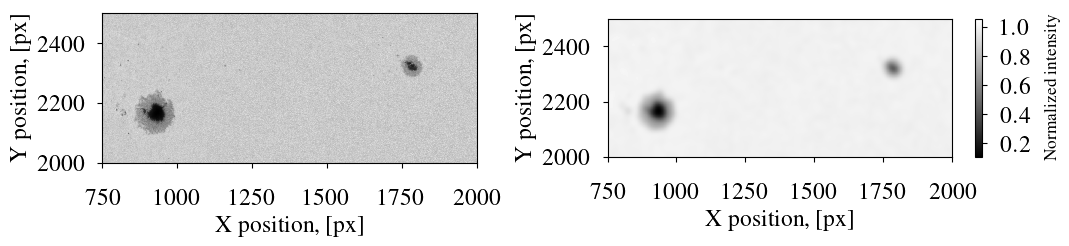
\includegraphics[scale = 0.600]{smth_spot}
%\includegraphics[scale = 0.735]{spt_smask}
%\caption[]{Mask given by Eq.~\eqref{eq:spt_mask} for the intensity image smoothed according to Eq.~\eqref{eq:smh} with
%           $\sigma_x = \sigma_y = 10 \mbox{px}$.
%           The pixels outside $r = 0.953R_\odot$ circumference (dashed line) have been disregarded.}
%\label{fig:spt_smask}
%\end{figure*}
%The comparison of the original and smoothed images is shown in the upper panels of Fig.~\ref{fig:spt_smask}, 
%the smoothed intensity mask built according to Eq.~\eqref{eq:spt_mask} is shown in the lower panel.
